\section{Experiment Design}
\label{sec:experiment}
Based on the design decisions, we developed a QS interface using a React.js frontend and a Next.js backend powered on MongoDB. Both systems are open-sourced~\footnote{link-to-github}.

We recruited participants from a midwestern college town using online ads, digital bulletins, social media posts, physical flyers, and online newsletters. The study's researcher prioritized the non-student population to maximize participant diversity. When recruiting participants, we did not reveal that the goal of this study is to measure their cognitive load and study their behaviors, rather a study that elicit community members' attitudes on societal issues. The reason we witheld such information is to prevent response biases. This study is reviewed and approved by the college Institutional Review Board.

\begin{figure}[ht]
    \centering
    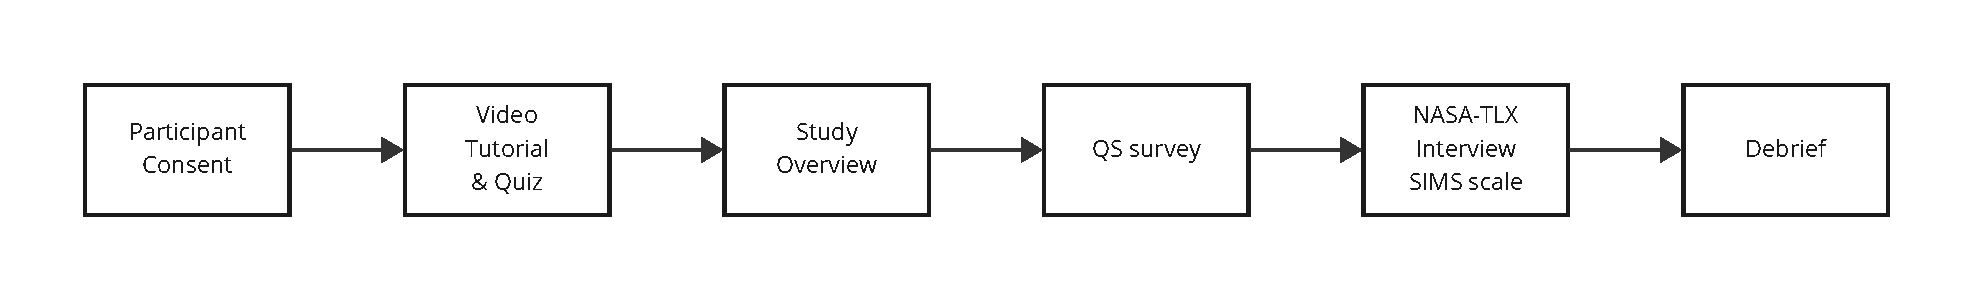
\includegraphics[width=1\textwidth]{content/image/study_flow.pdf}
    \caption{Study protocol}
    \label{fig:studyProtocol}
\end{figure}

Figure~\ref{fig:studyProtocol} shows a visual representation of the study protocol. Study participants are invited to the lab to participate in this study. The reason we made this experiment design decision is to minimize the influence of external factors that could affect the measurement of cognitive load. External factors, more prevalent in remote experiments or those conducted via platforms like MTurk, include potential multitasking or interruptions by others. An in-lab study also allows participants to operate across a consistent device that researchers have full control over. More specifically, the experiment involves participants operating on a 32-inch vertical monitor. This setup assured study participants, despite any condition in the study, can see all options on a QS, minimizing hidden information from an individual's decision-making process.

After consenting to the study, participants are invited to the study and they watch a pre-recorded video explaining the Quadratic mechanism and how QS operates. This video does not include any hints of either interface and how to operate the interface. Participants are then asked to complete a short quiz. The purpose of the quiz is to ensure that all participants fully understand how QS works. Participants are not screened out if they fail the quiz but are asked to rewatch the video or ask the researcher until they are able to select the correct answer. The device that the participant worked on is screen captured throughout the study.

The researcher then primes the participant that the purpose of this study is to assist local community organizers in understanding community members' preferences on a wide variety of societal issues so they can potentially distribute limited resources better. Participants would be randomly placed into one of the four groups:

\begin{itemize}
    \item 6 options with a text-based interface
    \item 6 options with an interactive interface
    \item 24 options with a text-based interface
    \item 24 options with an interactive interface
\end{itemize}

Participants will begin completing the survey independently, without the researcher's presence. Upon completion, they contact the researcher, who then requests they complete the NASA-TLX to assess cognitive load. This is followed by a short semi-structured interview to gain insights into the participants' experiences. This interview is audio recorded. Finally, participants complete the situational motivation scale (SIMS) to gauge motivation and a demographic survey. The session concludes with a debriefing and a \$15 cash compensation for their participation. The debreifing explains to the participant regarding not disclosing the purpose of the survey is to measure cognitive load and interface design and allows for participants to ask any questions.

The study is designed as a between-subject study for two reasons. First, we aim to minimize the study fatigue that might occur given the complexity of responding to a QS. To complete a QS survey, participants can take up to 20 minutes. Thus, it is difficult to conduct back-to-back experiments that measure cognitive load. We choose not to ask participants to revisit the lab with several days in between, to reduce dropout rates and prevent demotivating participants from attending the in-person experiment, which might occur in a within-subject study design. Second, we aim to reduce the learning effect that is difficult to remove, especially concerning operating the interface and making decisions on the survey. Recall that preferences are constructed, we want to ensure that participants are not influenced by their previous preferences which can influence their perceived cognitive load.

In an ideal world, understanding participants' cognitive load across multiple options would require enumerating all possible numbers of options and eliciting the ``breaking point'' where the participant experiences cognitive overload. Unfortunately, this is not feasible. Iterating through all possible numbers of options is very costly, both in time and resources. Therefore, we refer to prior literature to inform our choice of 6 and 24 options, representing a short and long list of options. To decide the number for the short list, survey methods such as constant sum surveys and Analytic Hierarchy Process (AHP) recommend options fewer than ten and seven, respectively~\cite{moroneyQuestionnaireDesignHow2019, saatyGroupDecisionMaking2013, saatyPrinciplesAnalyticHierarchy1987}. However, we are not aware of any specific works that justify these numbers.~\textcite{saatyPrinciplesAnalyticHierarchy1987} associated this value with both the cognitive processing capacity of $7\pm2$~\cite{millerMagicalNumberSeven1956} and a theoretical proof using the consistency ratio of a pairwise comparison metric~\cite{saaty2003magic}. This informs our decision to contain a pair of dependent variables above and below seven options. We turn to experiments designed to study choice overload. A meta-analysis by~\textcite{chernevChoiceOverloadConceptual2015} surveyed 99 choice overload experiments (N = 7202) and summarized that 6 and 24 are the modal values for short and long lists when testing choice overload. These two values are likely rooted in the original choice overload experiment by~\textcite{iyengarWhenChoiceDemotivating2000}. The value six is often used in experiments to understand the effect of choice provision. The value 24 is the maximum number of ecologically valid jams produced by the jam company in the original study. We decided to follow suit with these two values, satisfying the previous decision to choose two values less than and greater than seven.

Next, we describe the context of the survey that participants completed. Participants were asked to complete a societal issue survey. We follow suit as described by~\textcite{chengCanShowWhat2021}, believing that surveying societal issues is a good topic as it is relevant to every citizen and it is easy to convey that there are limited resources in the public sector to be prioritized across different sectors and areas. Participants across all four groups were presented with options randomly drawn from 26 societal issues. These issues were generated from the categories used by Charity Navigator~\cite{CharityNavigatorAnimals2023}, a non-profit organization that evaluates over 20 thousand charities in the United States. The full list of these societal issues is provided in Appendix B.

Last, we describe the two quantitative measurements taken during the study: cognitive load and motivation. At the time of this study, several methods existed to measure cognitive load, including performance measures, psychophysiological measures, subjective measures, and analytical measures~\cite{gaoMentalWorkloadMeasurement2013}. Given the nature of QS, a task requiring a long period, adopting performance measures like secondary-task measures in our experiment proved challenging due to the difficulty of designing a secondary task. The secondary task must use the same cognitive resources as the primary tasks, and the cognitive resource for completing the survey would vary among participants. Similarly, psychophysiological measures such as pupil size~\cite{palinkoEstimatingCognitiveLoad2010} and ECG~\cite{haapalainenPsychophysiologicalMeasuresAssessing2010} can be highly sensitive to external environments and costly to obtain. Consequently, we relied primarily on subjective measures via self-report surveys and analytical measures like time and clicks collected via the interface. We adopted a paper-based weighted NASA Task Load Index (NASA TLX), a multidimensional scoring procedure using the weighted average of six subscale scores to represent overall workload. Weighted NASA-TLX uses a priori workload definitions from subjects to weight and average subscale ratings, requiring subjects to evaluate each weight's contribution to the workload of a specific task~\cite{hart1988development, hartNasaTaskLoadIndex2006, cain2007review}. This approach reduces between-rater variability, indicating differences in workload definitions among raters within a task and variations in workload sources between tasks~\cite{cain2007review}. Despite criticisms regarding its validity and vulnerability, NASA-TLX is commonly used due to its low cost and ease of administration~\cite{gaoMentalWorkloadMeasurement2013}. It has been tested on various experimental and lab tasks, and workload scores derived from these tests showed significantly less variability among evaluators than one-dimensional workload scores~\cite{rubioEvaluationSubjectiveMental2004}. Thus, we chose NASA-TLX to measure cognitive load in our study.

In addition to NASA-TLX, we administered a situational motivation scale (SIMS) to measure participants' motivation (required citation). We posited that motivation would influence mental demand (required citation). SIMS, chosen for its widespread use, helps understand one's intrinsic motivation, extrinsic motivation, identified regulation, and external regulation, and was originally designed to measure self-determination. Both instruments were administered using pen-and-paper.
